\newpage
\hypertarget{static:starting vis}{}
\subsection{Getting started in EA}
\visHeader
  
\begin{itemize}

\item[$\blacktriangleright$]  To begin, navigate to ``New Metamodel Project''(Fig.~\ref{eclipse:newVisModelButton}) and start a new project named \texttt{Leit\-ners\-Learn\-ing\-Box} (Fig.~\ref{eclipse:newVisModel}). Open the empty \texttt{.eap} file in EA.

\vspace{0.5cm}

\begin{figure}[htbp]
	\centering
  
\includegraphics[width=0.3\textwidth]{eclipse_visNewMetamodelButton}
	\caption{``New Metamodel Project'' button}
	\label{eclipse:newVisModelButton}
\end{figure}
\begin{figure}[htbp]
	\centering
  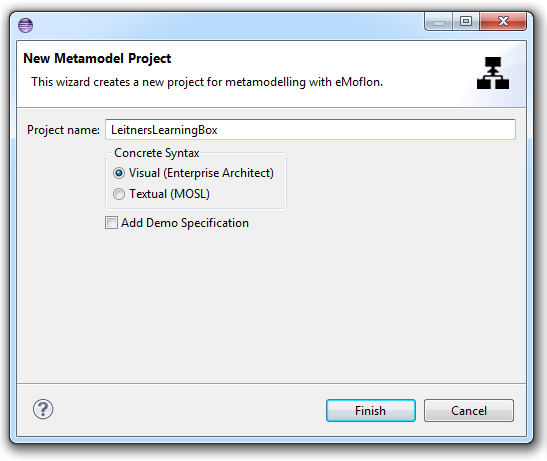
\includegraphics[width=0.8\textwidth]{eclipse_visNewMetamodelPlain}
	\caption{Starting a new visual project}
	\label{eclipse:newVisModel}
\end{figure}

\vspace{0.5cm}

\item[$\blacktriangleright$] In EA, select your working set and press the ``Add a Package'' button (Fig.~\ref{ea:newPackage}). 

\begin{figure}[htbp]
	\centering
  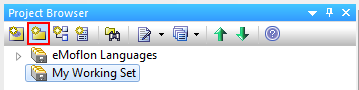
\includegraphics[width=0.5\textwidth]{ea_addPackage}
	\caption{Add a new package to \texttt{MyWorkingSet}}
	\label{ea:newPackage}
	\vspace{0.5cm}
\end{figure}

\clearpage

\item[$\blacktriangleright$] In the dialogue that pops up (Fig.~\ref{ea:newPackageName}), enter \texttt{LearningBoxLanguage} as the name of the new
package. In this case select \texttt{Package Only} and click \texttt{OK}. Later you can select \texttt{Create Diagram} to skip the next step.

\vspace{0.5cm}

\begin{figure}[htbp]
	\centering
    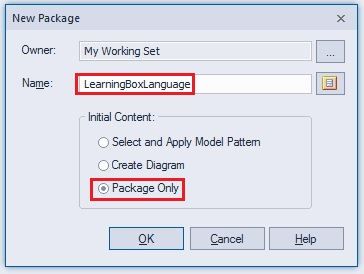
\includegraphics[width=0.6\textwidth]{ea_nameEPackage}
	\caption{Enter the name of the new package}
	\label{ea:newPackageName}
\end{figure}
\FloatBarrier

\vspace{0.5cm}

\item[$\blacktriangleright$] Your \texttt{Project Browser} should now resemble Fig.~\ref{ea:newPackageComplete}.

\vspace{0.5cm}

\begin{figure}[htbp]
	\centering
  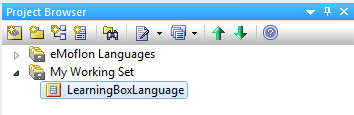
\includegraphics[width=0.5\textwidth]{ea_newPackage}
	\caption{State after creating the new package}
	\label{ea:newPackageComplete}
\end{figure}
\FloatBarrier

\vspace{0.5cm}

\item[$\blacktriangleright$] Now select your new package and create a ``New Diagram'' (Fig.~\ref{ea:newDiagram}).

\vspace{0.5cm}

\begin{figure}[htbp]
	\centering
  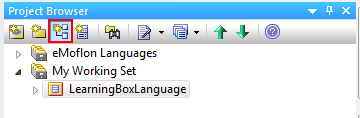
\includegraphics[width=0.5\textwidth]{ea_addDiagram}
	\caption{Add a diagram}
	\label{ea:newDiagram}
\end{figure}
\FloatBarrier

\clearpage

\item[$\blacktriangleright$] In the dialogue that appears (Fig.~\ref{ea:diagramType}), choose \texttt{eMoflon Ecore Diagrams} and press \texttt{OK}. 

\begin{figure}[htbp]
	\centering
  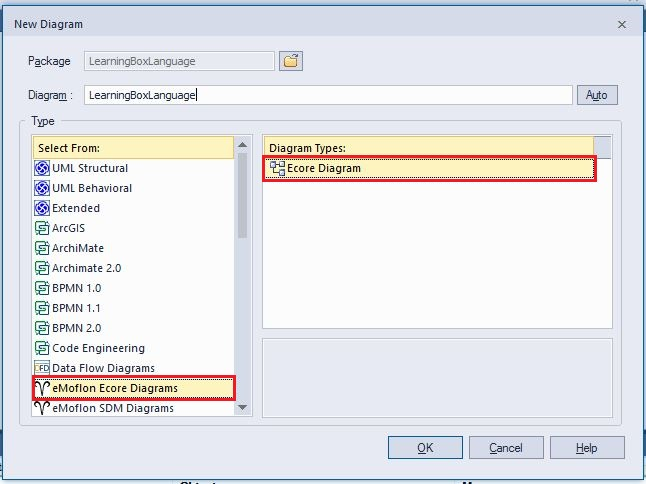
\includegraphics[width=0.9\textwidth]{ea_chooseDiagramType}
	\caption{Select the ecore diagram type}
	\label{ea:diagramType}
\end{figure}
\FloatBarrier

 
\item[$\blacktriangleright$] After creating the new diagram, your  \texttt{Project Browser} should now resemble Fig.~\ref{ea:diagramComplete}. You'll notice
that your \texttt{LearningBoxLanguage} package has been transformed into an EPackage.

\begin{figure}[htbp]
	\centering
  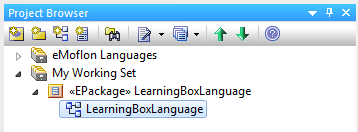
\includegraphics[width=0.5\textwidth]{ea_afterDiagramState}
	\caption{State after creating diagram}
	\label{ea:diagramComplete}
\end{figure}
\FloatBarrier

\item[$\blacktriangleright$] You can now already export your project to Eclipse,\footnote{If unsure how to perform this step, please refer to Part I, Section
2.1} then refresh your \texttt{Package Explorer}. A new node, \texttt{My Working Set}\footnote{If you do not have the two distinct nodes, ensure your ``Top
Level Elements'' are set to \texttt{Working Sets}} should have appeared containing your EPackage (Fig.~\ref{eclipse:initExport}). You can see that a
\texttt{LearningBoxLanguage.ecore} file has been generated, and placed in ``model.'' This is your metamodel that will contain all future types you create in
your diagrams.

\clearpage

\vspace*{2cm}

\begin{figure}[htbp]
	\centering
  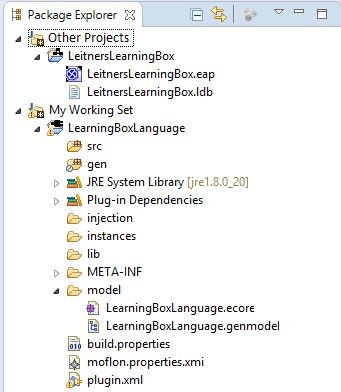
\includegraphics[width=0.55\textwidth]{eclipse_visInitExport}
	\caption{Initial export to Eclipse}
	\label{eclipse:initExport}
\end{figure}

\vspace{1cm}

\item[$\blacktriangleright$] If you're interested in reviewing the overall project structure and the purposes of certain files and folders, read Section 4.1
from Part~I. Otherwise, continue to the next section to learn how to declare classes and attributes.

\jumpSingle{static:classes vis}

\end{itemize}
